\documentclass{article}
\usepackage{amsmath}
\usepackage{amsthm}
\usepackage{amssymb}
\usepackage{enumerate}
\usepackage{tikz}
\usepackage{graphicx}

\begin{document}
  \title{Exercise 15.3}
  \author{Wang Yue from CS Elite Class}
  \date{\today}
  \maketitle

  \subsection*{24. }
  
  $$\begin{aligned}
    \int_0^4 \int_{-\sqrt x}^{\sqrt x} (1 + x^2y^2) dy dx &= \int_0^4 2 \int_0^{\sqrt x}(1+x^2y^2) dy dx \\
    &= \int_0^4 2 (y + x^2 \frac{y^3}{3})\biggl|_{y = 0}^{y = \sqrt x} dx \\
    &= \int_0^4 (2\sqrt x + \frac{x^{\frac 7 2}}{3}) dx \\
    &= (\frac 4 3 x^{\frac 3 2} + \frac{2}{27} x^{\frac 9 2})\biggl|_0^4 \\
    &= \frac{32}{3} + \frac{1024}{27} \\
    &= \frac{1312}{27}
  \end{aligned}$$

  \subsection*{40. }

  $$\begin{aligned}
    & \int_{-1}^1 \int_{-\sqrt{1-x^2}}^{\sqrt{1-x^2}}(8 - x^2 - 2y^2 - 2x^2 - y^2) dy dx \\
    &= \int_{-1}^1 \int_{-\sqrt{1-x^2}}^{\sqrt{1-x^2}}(8 - 3x^2-3y^2)dydx \\
    &= \int_0^{2\pi} \int_0^1 (8r - 3r^3) dr d\theta \\
    &= \int_0^{2\pi} (4r^2 - \frac{3r^4}{4})\biggl|_0^1 d\theta \\
    &= \int_0^{2\pi} (4 - \frac 3 4) d\theta \\
    &= \frac{13\pi}{8}
  \end{aligned}$$

  \subsection*{49. }

  $$\begin{aligned}
    \int_0^1 \int_{3y}^3 e^{x^2} dx dy &= \int_{0}^3 \int_0^{\frac x 3} e^{x^2}dydx \\
    &= \int_0^3 \frac x 3 e^{x^2} dx \\
    &= \int_0^3 \frac 1 6 e^{x^2} dx^2 \\
    &= \frac 1 6 e^{x^2}\biggl|_0^3 \\
    &= \frac{e^9 - 1}{6}
  \end{aligned}$$

  \subsection*{53. }

  $$\begin{aligned}
    \int_0^1 \int_{\arcsin y}^{\frac \pi 2}\cos x \sqrt{1+\cos^2 x} dx dy &= \int_0^{\frac \pi 2} \int_0^{\sin x} \cos x \sqrt{1+\cos^2 x} dy dx \\
    &= \int_0^{\frac \pi 2} \sin x \cos x \sqrt{1+\cos^2 x} dx \\
    &= -\frac 1 2 \int_0^{\frac \pi 2}\sqrt{1+\cos^2 x} d(1 + \cos^2 x) \\
    &= -\frac 1 2 \times \frac 2 3 (1 + \cos^2 x)^{\frac 3 2}\biggl|_{0}^{\frac \pi 2} \\
    &= -\frac 1 3 (0 - 1) \\
    &= \frac 1 3
  \end{aligned}$$
  \subsection*{54. }

  $$\begin{aligned}
    \int_0^8 \int_{\sqrt[3] y}^2 e^{x^4} dx dy &= \int_0^2 \int_0^{x^3} e^{x^4} dy dx \\
    &= \int_0^2 x^3 e^{x^4} dx \\
    &= \frac 1 4 \int_0^2  e^{x^4} dx^4 \\
    &= \frac 1 4 e^{x^4}\biggl|_0^2 \\
    &= \frac{e^{16} - 1}{4}
  \end{aligned}$$

  \subsection*{62. }

  $$D = \{ (x, y) | x \geq 0 \textrm{ and } y \geq \frac x 2 \textrm{ and } y \leq 3 - x \}$$

  \begin{center}
    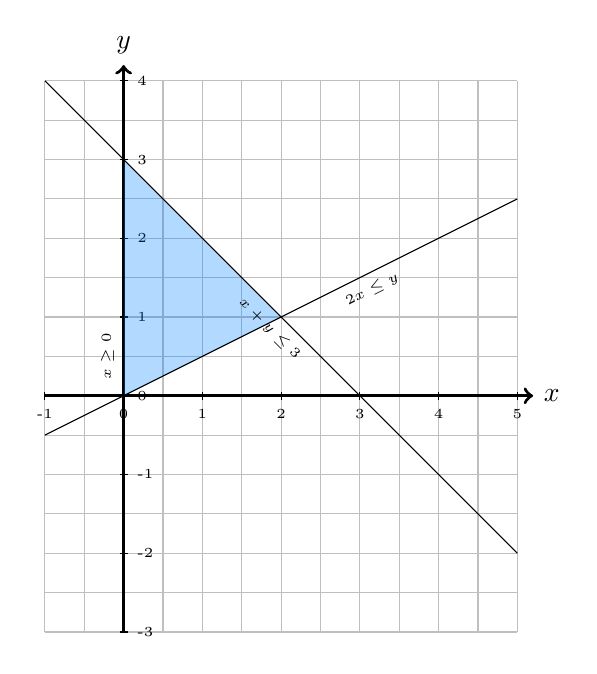
\begin{tikzpicture}

        \draw[gray!50, thin, step=0.5] (-1,-3) grid (5,4);
        \draw[very thick,->] (-1,0) -- (5.2,0) node[right] {$x$};
        \draw[very thick,->] (0,-3) -- (0,4.2) node[above] {$y$};

        \foreach \x in {-1,...,5} \draw (\x,0.05) -- (\x,-0.05) node[below] {\tiny\x};
        \foreach \y in {-3,...,4} \draw (-0.05,\y) -- (0.05,\y) node[right] {\tiny\y};

        % \fill[blue!50!cyan,opacity=0.3] (8/3,1/3) -- (1,2) -- (13/3,11/3) -- cycle;
        \fill[blue!50!cyan,opacity=0.3] (0,0) -- (0,3) -- (2,1) -- cycle;

        \draw (-1,-0.5) -- (2,1) -- node[below left,sloped] {\tiny$2x\leq y$} (5,2.5);
        \draw (-1,4) -- node[below,sloped] {\tiny$x+y\leq3$} (5, -2);
        \draw (0,-3) -- node[above,sloped] {\tiny$x\geq0$} (0,4);

    \end{tikzpicture}
  \end{center}

  $$\iint_D f(x, y) dA = \int_0^2 \int_{\frac x 2}^{3-x} f(x, y) dy dx$$

  \subsection*{63. }

  $$\begin{aligned}
    \iint_D (x + 2) dA &= \int_0^3 \int_{-\sqrt{9-y^2}}^{\sqrt{9-y^2}}(x + 2) dx dy \\
    &= \int_0^3 (\frac{x^2}{2} + 2x)\biggl|_{x=-\sqrt{9-y^2}}^{x=\sqrt{9-y^2}} dy \\
    &= 4\int_0^3 \sqrt{9-y^2} dy \\
    &= 4 \times \frac{3^2\pi }{4} = 9\pi
  \end{aligned}$$
  \subsection*{66. }

  $$\begin{aligned}
    &\iint_D (2 + x^2y^3 - y^2 \sin x) dA \\
    &= \int_{-1}^{0}\int_{-y-1}^{y+1}(2 + x^2y^3-y^2\sin x)dx dy + \int_{0}^{1} \int_{y-1}^{1-y}(2 + x^2y^3-y^2\sin x) dx dy \\
    &= \int_{-1}^0 [4(y+1) + \frac{2(y+1)^3 y^3}{3}] dy + \int_0^1 [4(1-y) + \frac{2(1-y)^3 y^3}{3}] dy \\
    &= \int_{-1}^0 4(y+1) dy + \int_0^1 4(1-y) dy + \frac 2 3 \int_0^1 (1-y)^3 y^3 dy + \frac 2 3 \int_{-1}^0 (y+1)^3y^3dy \\
    &= 4(\frac{y^2}{y} + y)\biggl|_{-1}^0 + 4(y - \frac{y^2}{2})\biggl|_0^1 + \frac 2 3 (\frac{y^4}{4} - \frac{3y^5}{5} + \frac{3y^6}{6} - \frac{y^7}{7})\biggl|_0^1 + (\frac{y^7}{7} + \frac{3y^6}{6} + \frac{3y^5}{5} + \frac{y^4}{4})\biggl|_{-1}^0 \\
    &= 4 + \frac 2 3 (\frac 1 4 - \frac 3 5 + \frac 1 2 - \frac 1 7 + \frac 1 7 - \frac 1 2 + \frac 3 5 - \frac 1 4) \\
    &= 4
  \end{aligned}$$

\end{document}
